\documentclass[letterpaper,12pt,fleqn]{article}
\usepackage{matharticle}
\usepackage{pgfplots}
\pgfplotsset{compat=1.14}
\pagestyle{plain}
\begin{document}

\begin{center}
\Large Math-1003b Exam \#2
\end{center}

\vspace{0.5in}

Name: \rule{4in}{1pt}

\vspace{0.5in}

This exam is closed book and notes. You may use a scientific calculator; however, no
other electronics are allowed. Show all work; there is no credit for guessed answers. All
answers must be in factored form, where appropriate. All numerical answers must be
expressed using exact values, unless you are specifically asked for an approximate
(decimal) value. All intervals must be expressed in interval notation.

\vspace{0.25in}

\begin{enumerate}
\item A new rock band is performing at the SJSU event center. The band wants to spread
  some posters around town advertising the performance. The printer says that the cost
  to print each poster varies directly with the area of the poster and inversely with
  the number of posters ordered.
  \begin{enumerate}
  \item Let $p=$ the cost to print each poster, $A=$ area of each poster and $n=$ number
    of posters printed. Write an equation that expresses the cost of each poster in terms
    of $A$ and $n$.

    \vspace{1in}

  \item What is the value of the constant of proportionality if the price per poster is
    \$4 when printing 100 posters of size 80 square inches each?

    \vspace{1.25in}

  \item The band decides that they would like the posters to be a bit bigger and that
    they don't need 100 of them. How much is the price per poster when printing 80
    posters of size 160 square inches each?
  \end{enumerate}

  \newpage

\item Solve the compound inequality for $x$:
  \[-6<-2(x-1)-5\le2\]

  \vspace{3in}

\item Solve the following system of inequalities for $x$:
  \[-3(x-7)>15\hspace{2ex}\mbox{or}\hspace{2ex}x+2\le5\]

  \newpage

\item Solve for $x$. Your work must include a test point table for full credit:
  \[x^2+2x-15>0\]

  \vspace{3in}

\item Solve for $x$. Your work must include a test point table for full credit:
  \[\frac{x+1}{x-2}\le0\]

  \newpage
  
\item Solve for $x$:
  \[2\abs{3x-1}-2=6\]

  \vspace{4in}

\item Solve for $x$:
  \[\abs{5x+3}=-2\]

  \newpage

\item Solve for $x$:
  \[2\abs{7x-1}+4\le6\]

  \vspace{3.5in}

\item Solve for $x$ (Hint: Look at the previous problem):
  \[2\abs{7x-1}+4>6\]

  \newpage

\item Solve the following system of inequalities by graphing. Be sure to label all key
  points and make it absolutely clear which region(s) of the plane you are selecting for
  your answer:
  \[\left\{\begin{array}{l} x+y>3 \\ y\le1 \end{array}\right.\]
  
  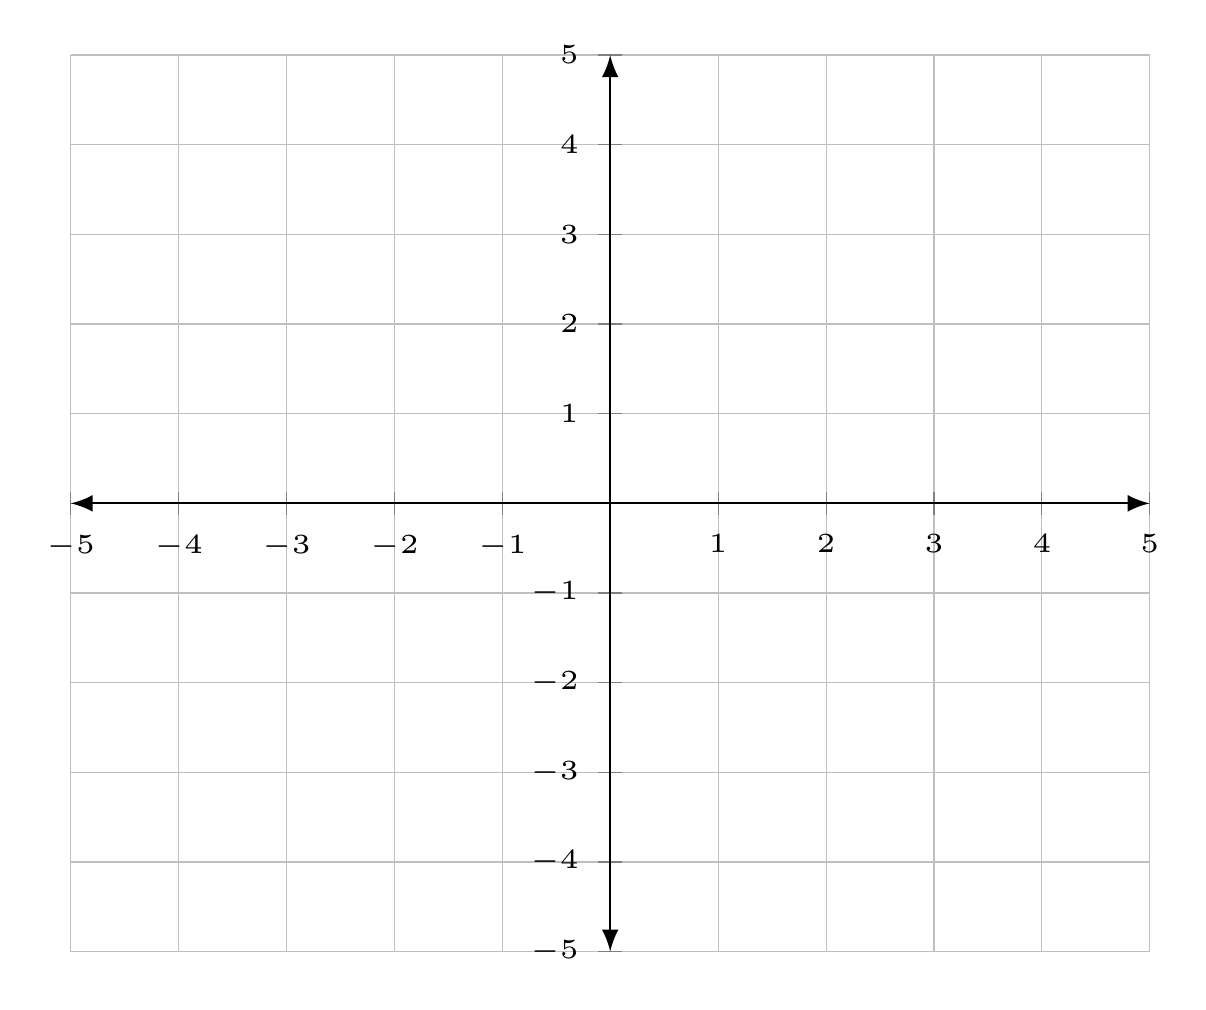
\begin{tikzpicture}[scale=2]
    \begin{axis}[
        xmin=-5,xmax=5,
        ymin=-5,ymax=5,
        grid=both,
        grid style={line width=.1pt, draw=gray!10},
        major grid style={line width=.2pt,draw=gray!50},
        axis lines=middle,
        axis line style={latex-latex},
        xtick={-5,-4,-3,-2,-1,0,1,2,3,4,5},
        ytick={-5,-4,-3,-2,-1,0,1,2,3,4,5},
        ticklabel style={font=\tiny},
      ]
    \end{axis}
  \end{tikzpicture}

\end{enumerate}

\end{document}
